\documentclass[exam,addpoints, noanswers]{exam}

\usepackage[exam]{physics9}

\title{Practice Test \#4B}
\date{\today}
\author{\mobeardInstructorShort}

\begin{document}
\maketitle
\vfill
\mobeardExamNameBlock
\vfill
Instructions: 
\begin{enumerate}
\item Do not open exam until instructor announces that you may begin.
\item Please write your name on each page in case the sheets are separated. 
\item Closed notes, closed book.  You may use two \SI{8.5x11}{\inch} note hardcopy sheets, both sides. You may NOT use your computer or phone as your notes. 
\item Calculators (TI-84 or equivalent) are permitted.  On standardized tests you will not be permitted to use your cell phone as a calculator, so it is best to get used to your calculator now. You may NOT use your computer or phone as your calculator. 
\item Eight multiple choice are worth five points each, three essay questions (divided into parts) are worth 20 points each. 
\item In answering the essay questions, be thorough but concise. Deep understanding of the concepts will be displayed by proper use of vocabulary and discussion of the interconnectedness of concepts. 
\item Show your calculations and (most importantly) your \textbf{thinking}.
\end{enumerate}
\vfill
\begin{center}
\gradetable[h][questions]
\end{center}
\clearpage



\begin{questions}
\question[5] Easy warmup question: what are the correct SI units for mass? 
\begin{choices}
\CorrectChoice \si{\kilo\gram}
\choice pound
\choice slug
\choice long ton
\end{choices}

\question[5] Two 6S racing quadrotors (mass \SI{700}{\gram}) are heading straight towards each other (head on) at 165 mph (\SI{74}{\meter\per\second}). What is the total momentum of the system? 
\begin{choices}
\CorrectChoice Zero, since they are heading straight towards each other 
\choice \SI{104}{\kilo\gram\meter\per\second}
\choice \SI{10400}{\kilo\gram\meter\per\second}
\choice Zero, because momentum is conserved
\end{choices}

\question[5] Which of the following are situations in which you might expect (linear) momentum to be conserved? Please select all that apply. 
\begin{choices}
\choice A cart being accelerated by current a magnetic field
\choice A super spy freefalling from a blimp
\choice A yellow labrador retriever accelerating as he runs to catch a ball
\choice An F-18 being decelerated by an arrestor cable
\choice A baseball orbiting the earth 
\end{choices}

\question[5] Which do you expect to have the most momentum?
\begin{choices}
\choice A stationary blue whale (\emph{Balaenoptera musculus})
\choice A \emph{\dag Baluchitherium} moving at \SI{0.00001}{\milli\meter\per\second}
\choice A stationary \emph{\dag Diplodocus}
\choice A stationary mouse (\emph{Mus musculus})
\choice A mouse fired from an air cannon at \SI{30}{\meter\per\second}
\end{choices}

\clearpage
\question[5] A Canadian physicist is explaining something to you and mentions that it is like what happens during curling (``chess on ice'') when a puck collides with another puck. You may not know much about curling but what physics do you think the Canadian is alluding to? 
\begin{choices}
\CorrectChoice momentum conservation during an elastic collision
\choice momentum conservation during an inelastic collision
\choice quantum entanglement of pucks created in the same event
\choice repulsion due to electric fields
\choice nuclear fusion
\end{choices}

\question[5] Two bighorn sheep (\emph{Ovis canadensis}, mass \SI{68}{\kilo\gram} each) run head on at each other at \SI{11}{\meter\per\second}. For a single sheep, what is the change in momentum? 
\begin{choices}
\CorrectChoice \SI{748}{\kilo\gram\meter\per\second}
\choice Zero, since they are running head on at each other
\choice Zero, since momentum is conserved
\choice \SI{8000}{\newton}
\choice \SI{0.1}{\second}
\end{choices}

\question[5] Xuan the puppy walks one block east, one block north, one block west, and one block south. What is the distance Xuan traveled? 
\begin{choices}
\CorrectChoice four blocks
\choice zero blocks
\choice one block
\choice half a block east and half a block north
\choice one block in each direction
\end{choices}

\question[5] A scientist decides to model the impact of a wave traveling at velocity $v$ on a stationary surfer of mass $m$. They argue the equivalent mass after the impact is about $2m$, and thus the velocity of the surfer immediately after the impact is about $\frac{v}{2}$. What assumption is the scientist making? Please select all that apply
\begin{choices}
\CorrectChoice The scientist is assuming the impact can be modeled as an inelastic collision
\CorrectChoice The scientist is assuming inviscid flow
\choice The scientist is assuming low Reynolds number flow
\choice The scientist is assuming compressible flow
\choice The scientist is assuming the impact can be modeled as an elastic collision
\end{choices}




\clearpage
\question\label{q9} The Mars Helicopter Ingenuity (\fref{fig:q9}) is a small (\SI{1.8}{\kilo\gram}) solar-powered helicopter with counter-rotating blades that spin at about \SI{2400}{\rpm}. It is equipped with computers, navigation sensors, and two cameras. The height is \SI{0.49}{\meter} and the span is \SI{1.2}{\meter}. It is deployed from the Mars Rover Curiosity (\SI{899}{\kilo\gram}). 
\begin{figure}[h]
\begin{center}
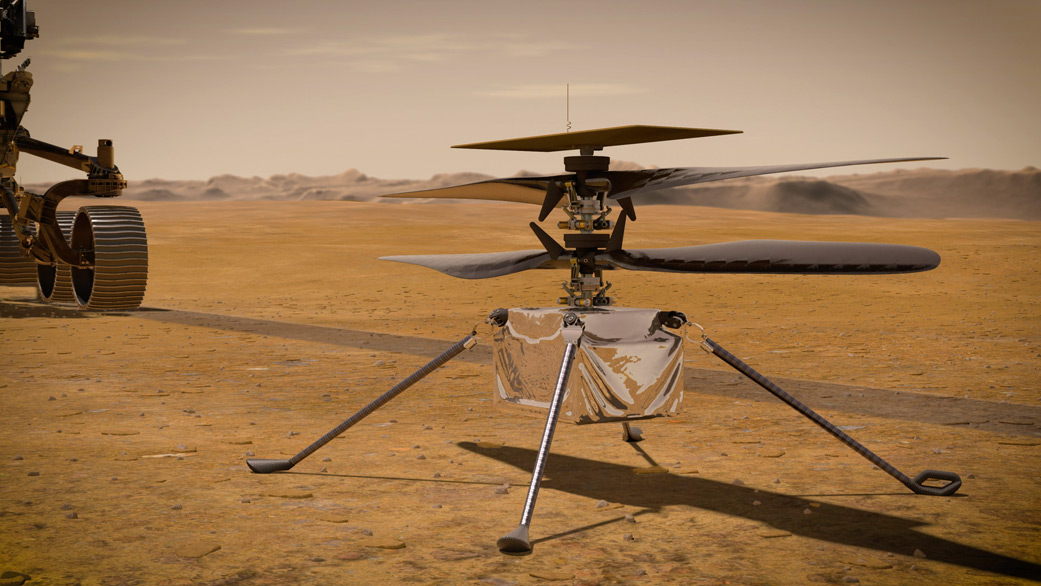
\includegraphics[width=1.5in]{ingenuity.jpg}
\end{center}
\caption{Question~\ref{q9}}
\label{fig:q9}
\end{figure}
\begin{parts}
\part[5] Assume the Ingenuity has taken off, is out of ground effect, and is translating steadily upwards at \SI{0.5}{\meter\per\second}. Draw a free body diagram of the Mars Helicopter Ingenuity.
\begin{solution}[3in]
\end{solution}

\part[5] If the acceleration of gravity on Mars is \SI{-3.38}{\meter\per\second\squared}, what is the weight of the Mars Helicopter Ingenuity, and how much upward force must the rotors generate during this flight condition?
\begin{solution}[1.5in]
\end{solution}

\clearpage
\part[5] The onboard computers detect a fault and go into an emergency state where the craft descends under \textbf{autorotation}. During autorotation at the autorotation speed, the rotors ``windmill'' and generate enough lift to exactly counteract the weight. Draw a free body diagram of the Mars Helicopter Ingenuity during this state. 
\begin{solution}[3in]
\end{solution}

\part[5] If the acceleration of gravity on Mars is \SI{-3.38}{\meter\per\second}, what is the overall acceleration of the craft once it reaches the autorotation speed? 
\begin{solution}[1in]
\end{solution}
\end{parts}




\clearpage
\question For the second short answer question, you get a job at NASA working on a small, zero G robot propelled with compressed air, able to move around inside the International Space Station. You are planning a set of commands to transmit to the robot for an upcoming flight test on a ``Vomit Comet'' C-9B microgravity simulator plane. 

\begin{parts}
\part[10] The first test maneuver is to fly up \SI{1}{\meter} in \SI{1}{\second}, hover for 
\SI{1}{\second}, then return to the launch point in \SI{1}{\second}. In the space here, sketch the vertical position and velocity of the robot. (You will need this to construct velocity commands to send to the robot, and to set failsafe limits on position in its autonomous flight controller.) 
\begin{solution}[6in]
\end{solution}

\clearpage
\part[10] During the actual test, a failure occurs in the propulsion system, resulting in the throttle valve being stuck open during the first part of the maneuver (heading upwards). With the failed valve, the force on the robot is \SI{10}{\newton} and its mass is \SI{1}{\kilo\gram}. Please plot the robot's position versus time. The far wall of the test chamber is \SI{10}{\meter} away; show when it hits the wall on your graph. Assume the robot is streamlined so that air resistance is small and neglect any change in mass from the expulsion of propellant.  
\begin{solution}[6in]
\end{solution}
\end{parts}


\clearpage
\question
\begin{parts}
\part[10] In your own words, describe what is the difference between momentum and energy? 
\begin{solution}[4in]
\end{solution}
\part[10] In your own words, describe what is the difference between position, velocity, and acceleration? 
\begin{solution}[4in]
\end{solution}
\end{parts}
\end{questions}
\end{document}